\documentclass[a4paper]{article}
\usepackage[spanish]{babel}
\usepackage[utf8]{inputenc}
\usepackage{charter}   % tipografia
\usepackage{graphicx}
%\usepackage{makeidx}
\usepackage{paralist} %itemize inline
\usepackage{lstlisting}
%\usepackage{float}
%\usepackage{amsmath, amsthm, amssymb}
%\usepackage{amsfonts}
%\usepackage{sectsty}
%\usepackage{charter}
%\usepackage{wrapfig}
%\usepackage{listings}
%\lstset{language=C}


\usepackage{color} % para snipets de codigo coloreados
\usepackage{fancybox}  % para el sbox de los snipets de codigo

\definecolor{litegrey}{gray}{0.94}

% \newenvironment{sidebar}{%
% 	\begin{Sbox}\begin{minipage}{.85\textwidth}}%
% 	{\end{minipage}\end{Sbox}%
% 		\begin{center}\setlength{\fboxsep}{6pt}%
% 		\shadowbox{\TheSbox}\end{center}}
% \newenvironment{warning}{%
% 	\begin{Sbox}\begin{minipage}{.85\textwidth}\sffamily\lite\small\RaggedRight}%
% 	{\end{minipage}\end{Sbox}%
% 		\begin{center}\setlength{\fboxsep}{6pt}%
% 		\colorbox{litegrey}{\TheSbox}\end{center}}

\newenvironment{codesnippet}{%
	\begin{Sbox}\begin{minipage}{\textwidth}\sffamily\small}%
	{\end{minipage}\end{Sbox}%
		\begin{center}%
		\vspace{-0.4cm}\colorbox{litegrey}{\TheSbox}\end{center}\vspace{0.3cm}}



\usepackage{fancyhdr}
\pagestyle{fancy}

%\renewcommand{\chaptermark}[1]{\markboth{#1}{}}
\renewcommand{\sectionmark}[1]{\markright{\thesection\ - #1}}

\fancyhf{}

\fancyhead[LO]{Sección \rightmark} % \thesection\ 
\fancyfoot[LO]{\small{Alejandro Mignanelli, Facundo Barañao, Ian Sabarros}}
\fancyfoot[RO]{\thepage}
\renewcommand{\headrulewidth}{0.5pt}
\renewcommand{\footrulewidth}{0.5pt}
\setlength{\hoffset}{-0.8in}
\setlength{\textwidth}{16cm}
%\setlength{\hoffset}{-1.1cm}
%\setlength{\textwidth}{16cm}
\setlength{\headsep}{0.5cm}
\setlength{\textheight}{25cm}
\setlength{\voffset}{-0.7in}
\setlength{\headwidth}{\textwidth}
\setlength{\headheight}{13.1pt}

\renewcommand{\baselinestretch}{1.1}  % line spacing


% \setcounter{secnumdepth}{2}
\usepackage{underscore}
\usepackage{caratula}
\usepackage{url}


% ******************************************************** %
%              TEMPLATE DE INFORME ORGA2 v0.1              %
% ******************************************************** %
% ******************************************************** %
%                                                          %
% ALGUNOS PAQUETES REQUERIDOS (EN UBUNTU):                 %
% ========================================
%                                                          %
% texlive-latex-base                                       %
% texlive-latex-recommended                                %
% texlive-fonts-recommended                                %
% texlive-latex-extra?                                     %
% texlive-lang-spanish (en ubuntu 13.10)                   %
% ******************************************************** %



\begin{document}


\thispagestyle{empty}
\materia{Organización del Computador II}
\submateria{Primer Cuatrimestre de 2015}
\titulo{Trabajo Práctico III}
\subtitulo{El Kernel contraataca}
\integrante{Alejandro Mignanelli}{609/11}{minga_titere@hotmail.com}
\integrante{Facundo Barañao}{480/11}{facundo_732@hotmail.com}
\integrante{Ian Sabarros}{XXX/xx}{elgeniofederico@gmail.com}

\maketitle
\newpage

\thispagestyle{empty}
\vfill
\begin{abstract}
En el presente trabajo se describe el desarrollo del Kernel para una arquitectura intel de 32-bits, así como el manejo de paginación, manejo de tareas, interrupciones y todo lo referente al manejo de un pequeño sistema operativo.

\end{abstract}

\thispagestyle{empty}
\vspace{3cm}
\tableofcontents
\newpage

%\normalsize
\newpage

\section{Objetivos generales}

El objetivo de este trabajo práctico es, partiendo de un procesador intel de 32-bits, generar un kernel capaz de gestionar memoria entre diferentes tareas, correrlas de manera concurrente, y resolver las diferentes problemáticas que puedan surgir al momento de ejecución.

Para ello utilizaremos las diversas herramientas que intel pone a nuestra disposición en modo protegido: Usaremos segmentación y paginación para controlar el privilegio con el que las tareas se ejecutarán, además de limitar lo que las tareas puedan 'ver' con un mapeo parcial de la memoria.
Utilizaremos interrupciones del procesador que permitirán, tanto reaccionar de manera apropiada cuando se produzca un error en tiempo de ejecución, obtener input del teclado y gestionar un task manager que nos permita ejecutar tareas de manera concurrente.

En el presente informe, se detallará de manera más elaborada todo lo hecho para lograr el objetivo del trabajo práctico, así como cualquier decisión que se haya tomado en el código a tales fines. Para su mejor entendimiento, este informe se dividirá en ejercicios, que son pequeñas partes del trabajo, y todos juntos conforman al trabajo práctico en sí. 

\section{Ejercicio 1: GDT Basica}

\subsection{GDT básica y pasaje a modo protegido}

\begin{enumerate}

\item[a)] Completamos la GDT de la siguiente manera: El primer descriptor se completa con ceros, ya que este debe ser nulo siempre; las siguientes 7 entradas no se usan debido a que se consideran ocupadas; la octava y la novena entrada corresponden a un descriptor de código de nivel 0 y 3 respectivamente; las dos siguientes son descriptores de datos de nivel 0 y 3 respectivamente. Para un mejor entendimiento observar la figura "GDT".

Los descriptores de segmento de código llevan un 8 en su campo type (EXECUTE ONLY) mientras que los de datos llevan un 2 (READ/WRITE). Para lograr direccionar los primeros 500MB de memoria, establecemos el límite en {\tt 0x1F3FF} y la granularidad en 1.

\item[b)] En cuanto al pasaje a modo protegido, en primera instancia se deshabilitan las interrupciones ({\tt cli}) y se habilita el pin A20 para poder acceder a direcciones superiores al primer MB.  Luego se carga la GDT con la instrucci\'on {\tt lgdt} y la estructura {\tt gdt_descriptor} definida en {\tt gdt.h}. Lo siguiente es setear el bit PE del registro CR0 y hacer el salto mediante la instrucci\'on {\tt jmp} a la direcci\'on referenciada por la etiqueta {\tt modo_protegido} en la entrada 8 de la GDT, con nivel de privilegio 0.  Finalmente, se cargan los registros de segmento (DS, ES, GS y SS) y se establece la base de la pila de kernel en {\tt 0x27000}.

\item[c)] Asignamos la entrada 12 de la GDT para el área de pantalla. Se establece la base en {\tt 0xB8000} y su límite en {\tt 0x1000}, el campo type se define como 2 (READ/WRITE) y el bit S en 1. Una vez hecho esto, movemos el selector de esta entrada al registro de segmento FS.

\item[d)] Utilizamos la funcion {\tt inic_video} para limpiar la pantalla e inicializarla como muestra la figura \ref{fig:pantalla}. Hacemos uso de la estructura que se encuentra en {\tt screen.h} para ir asignando los distintos caracteres y sus atributos (color de caracter y su color de fondo). Para esto usamos la dirección física del buffer de video {\tt 0xB8000}.

\begin{figure}[h]
  \centering
    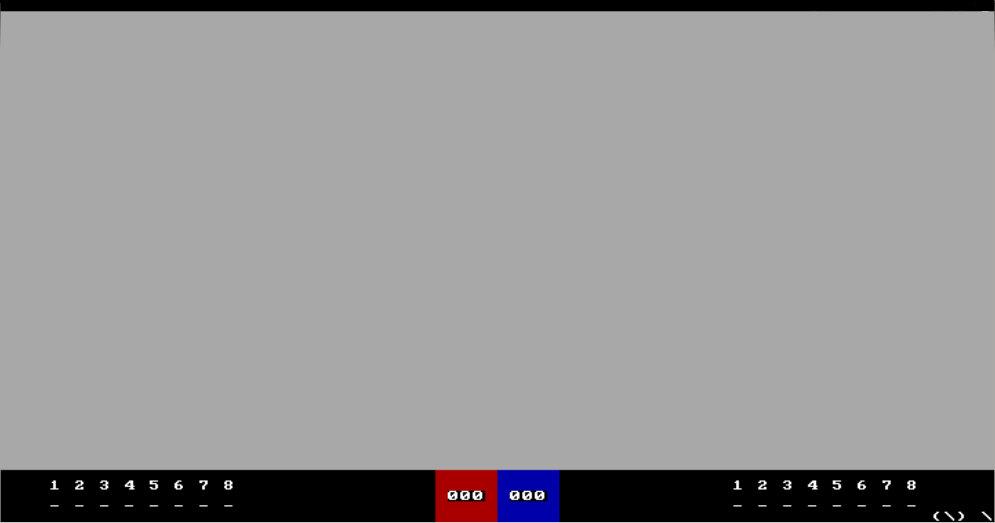
\includegraphics[width=0.75\textwidth]{imagenes/pantallainicial.png}
  \caption{Estado inicial de la pantalla}
  \label{fig:pantalla}
\end{figure}
 \FloatBarrier

\end{enumerate}

\section{Ejercicio 2: IDT Basica} 
\begin{enumerate}

\item[a)] Completamos la IDT con las primeras 19 entradas, que corresponden a diferentes rutinas de excepciones del procesador. Las excepciones reservadas por intel no son consideradas en este punto. Cargamos las entradas como {\it Interrupt Gate}; bit de presente en 1, DPL 00, bit de sistema en 0, tipo de puerta en 1 (32 bits) y el valor 110 en los bits 8-10. Por el momento, las rutinas de atención de excepciones estan hechas de manera tal que solo muestren por pantalla el error incurrido.

\item[b)] Cargamos la IDT agregando en {\tt kernel.asm} un call a {\tt idt\_inicializar} y usando la instrucción {\tt lidt} y la estructura {\tt idt\_descriptor} ya definida.  

\end{enumerate}



\section{Ejercicio 3: Paginación Basica}
\begin{enumerate}
\item[a)]Creamos la rutina {\tt inic_video} en {\tt screen.c}, esta sera la encargada de pintar la pantalla, limpiar el buffer de video e inicializar los valores en pantalla: ninguna tarea activa, puntajes nulos, mapa sin explorar. SACAR SCREENSHOT

\item[b)]Se escribe la rutina {\tt mmu_inicializar_dir_kernel} que como su nombre indica, inicializar el directorio y las tablas de páginas del kernel. Como es necesario mapear desde {\tt 0x00000000} a {\tt 0x003FFFFF} tendremos que utilizar una sola tabla de páginas. Esta se conecta con la primer entrada del directorio, la cual se encontrará presente, mientras que el resto de las entradas no lo estarán. El directorio de páginas se inicializa en la dirección {\tt 0x27000} mientras que la tabla se inicializa en {\tt 0x28000}. El mapeo lo realizamos con {\it identity mapping} dentro del rango establecido.

\item[c)]Una vez inicializados el directorio y las tablas de páginas, se procede a activar la paginaci\'on en {\tt kernel.asm}. Para esto se coloca en el registro {\tt cr3} la dirección base del directorio de páginas ({\tt 0x27000}), esto nos asegura que los bits {\tt PCD} y {\tt PWT} del registro están limpios, y finalmente se coloca en 1 el bit m {\tt PG} del registro {\tt cr0}.

\begin{lstlisting}[frame=single]
; Cargar directorio de paginas
mov eax, dir_kernel_addr ;0x27000
mov cr3, eax

; Habilitar paginacion
mov eax, cr0
or eax, 0x80000000
mov cr0, eax
\end{lstlisting}

\item[d)]Creamos la funcion {\tt imprime_nombre_grupo} en {\tt screen.c} que calcula el tamaño del string " Circus / Family " (función auxiliar {\tt long_string}) y en base a esto determina la posición que debe tener en la pantalla.





\section{Ejercicio 4: Memory Management Unit}
\begin{enumerate}
\item[a)] La rutina {\tt mmu_inicializar} en {\tt mmu.c} inicializa en 0 un contador de páginas ocupadas p\'aginas ocupadas, que se ir\'a incrementando en la medida en que se utilicen las p\'aginas, y llama a la funci\'on {\tt mmu_inicializar_dir_kernel}, previamente creada.\\
Contamos también con la función {\tt obtener_pagina_libre} que se encarga de incrementar el contador de páginas ocupadas y retornar el valor de una página libre reservada (estas páginas serán obtenidas del area libre del kernel). Para tratar de evitar problemas de solapamiento, resolvimos incrementar de a 2 el contador de páginas ocupadas, lo que terminaría en la reserva de 2 páginas. TAL VEZ HAY QUE CAMBIAR ESTO.

\item[b)] Se escribe la rutina {\tt mmu_inic_dir_pirata} para inicializar un directorio de páginas y tablas de páginas para una tarea. Esta función solo se encargará de inicializar el directorio de páginas y las tablas para un tarea, en lugar de tener que también copiar el código de la misma, responsabilidades que dejamos para otras funciones. Su funcionamiento resulta muy similar al de inicializar el directorio y las tablas para el kernel. Difiere en el hecho de que se debe pedir una página libre para el directorio y las tablas de páginas, devolviendo la dirección de la página pedida para el directorio.\\

Para el trabajo de copiar el c\'odigo del pirata y mapear las p\'aginas correspondientes, se crean las funciones {\tt copiar\_código} y {\tt mapear\_alrededores} en {\tt mmu.c}. La primera recibe como parámetros un cr3 (de la tarea cuyo código se quiere copiar), dos direcciones virtuales (una destino y otra origen) y una posicion pasada como 2 unsigned ints x e y (que serán pasadas como parámetros al código de la tarea). Esta función transforma las direcciones virtuales y con los otros parámetros antes mencionados llama a {\tt copiar\_fisico} la cual recupera el cr3Actual mediante la función {\tt rcr3}, mapea ambas direcciones fisicas (DST y SRC) a las direcciones {\tt 0x500000} y {\tt 0x501000} (direcciones que no tienen otro uso fuera de este) y tratandolas como punteros a int, se procede a copiar el código desde SRC a DST de a 4 bytes a la vez. Por último, {\tt copiar\_fisico} pasa los parámetros x e y a los últimos 8 bytes del destino y desmapea las 2 páginas mapeadas previamente. Para finalizar, mapeamos a la direccion {\tt 0x400000} la dirección física de destino.
La segunda función, {\tt mapear\_alrededores}, toma un cr3 sobre el cual realizar los mapeos y una dirección virtual Destino. Se pasa luego a transformar la dirección virtual a física y hacer los mapeos, teniendo en cuenta los cálculos correspondientes, para que se mapeen las 9 casillas ocupadas mantiendo una correspondencia entre direccion virtual y física.

\item[c)] Se crean las rutinas encargadas de mapear y desmapear páginas de memoria.

La rutina {\tt mmu\_mapear\_pagina} toma el valor de {\tt cr3} y la direccióon virtual, sobre la cual calcula los índices correspondientes a directorio y tablas de páginas. Luego accede a la entrada del directorio y procede de la siguiente manera: si esta entrada se encuentra como {\it presente}, se accede a la entrada correspondiente de tabla y se realiza el mapeo con la dirección física indicada; en caso contrario, primero se completa dicha entrada pidiendo una página libre y luego se hace el mapeo propiamente dicho.

La rutina {\tt mmu\_unmapear\_pagina} toma el valor actual de {\tt cr3} y la dirección virtual, de la cual calcula los índices correspondientes a directorio y tablas de páginas.  Luego accede a la entrada del directorio y, si estaba como {\it presente}, busca la entrada en la tabla de p\'aginas y la pone como {\it no presente}. En el caso de que ya se encontrar como {\it no presente} no hace ningún cambio.



\section{Ejercicio 5: Interrupciones De Teclado/Reloj}
\begin{enumerate}
\item[a)]Usaremos la entrada número 32 de la IDT para la interrupción de reloj, la número 33 para la interrupción de teclado y la número 70 para la interrupción de software {\tt 0x66}.  Las tres entradas se cargan como {\it interrupt gates}, y con los mismos atributos indicados en el apartado 2, con la diferencia de que a la 70 se le asigna el nivel de privilegio 3.

\item[b)]Se escribe una base para la rutina de atención. En esta instancia, el único objetivo de la rutina es llamar a la función {\tt screen_actualizar_reloj_global}, la cual se encarga de mostrar la animación de reloj por cada tick de reloj.

\item[c)]Definimos la base de la rutina de atención de teclado de manera que al presionar cualquier tecla, muestre un mensaje en la esquina superior derecha de la pantalla (llamando a {\tt imprime_tecla} definida en {\tt screen.h}). Esto se realiza para corroborar el buen funcionamiento de las interrupciones, alteraremos este aspecto. Luego de esto, la rutina llama a la función {\tt game_atender_teclado}, pasándole como parámetro el código de la tecla presionada. Esta se encarga de realizar la acción que corresponda dependiendo de la tecla indicada (lanzar explorador o activar debug).




\section{Ejercicio 6: TSS}
\begin{enumerate}

\item[a)]Definimos las entradas 13 (tarea inicial), 14 (tarea idle), 15-22 (tareas jugador 1), 23-30 (tareas jugador 2) de la GDT
A estas entradas se les asigna tipo 9 (Execute-Only,accessed), base 0, presente 1 y DPL 0. El límite se establece en {\tt 0x68} para que sea mayor al tamaño de una TSS. La Figura \ref{fig:gdt2} muestra el estado de la GDT luego de agregar estas entradas.

\begin{figure}[h]
	  \centering
	    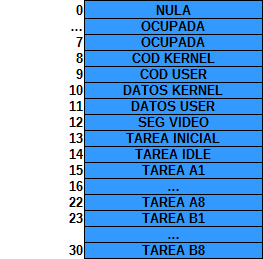
\includegraphics[ width=0.25\textwidth]{imagenes/gdt final.png}
	     \caption{Estado final de la GDT}
	  \label{fig:gdt2}
%	  \vspace{-15pt}
	\end{figure}
%	\FloatBarrier

\item[b)]Para completar la TSS de la tarea Idle hacemos uso de la función {\tt tss\_inicializar\_tarea\_idle}, la cual se encarga de asignar los segmentos de datos del kernel a los campos GS, FS, DS, SS, ES y poner el segmento de código de kernel en el campo CS. A su vez, completa ESP y EBP con la dirección del stack del kernel y se ocupa de que comparta el cr3 con el kernel. Por último, el EIP será {\tt 0x16000}, el campo EFLAGS se completa con {\tt 0x202} (para habilitar las interrupciones), el IOMAP con {\tt 0xFFFF} y el resto se deja en 0.

\item[c)] La función {\tt tss\_inicializar\_tareas\_piratas} toma como parámetro un puntero a tss y se ocupa de llenar sus campos. Los campos ES, SS, DS, FS y GS se completan con el segmento de datos de usuario, y el campo CS se completa con el segmento de código de usuario. Tanto ESP como EBP quedan seteados en {\tt 0x401000}, el campo EFLAGS en {\tt 0x202}, el CR3 en 0 (se le asignará un cr3 al momento de lanzar el pirata correspondiente utilizando la función {\tt mmu_inicializar_dir_tarea}), se pedirá una página nueva para el ESP0, SS0 se completa con segmento de datos kernel, IOMAP con {\tt 0xffff} y el resto con 0. 

\item[d)] En la rutina {\tt tss\_inicializar} pedimos una página libre para la tss de la tarea inical y asignamos la dirección obtenida en el campo {\it base} de la entrada correspondiente a esta tarea en la GDT.

\item[e)] En la rutina {\tt tss\_inicializar} completamos la entrada de la GDT perteneciente a la tarea Idle, completando el campo {\it base} con la dirección correspondiente a la misma.

\item[f)]Para pasar a la tarea IDLE primero se carga la tarea inicial en {\tt kernel.asm}, haciendo uso de la instruccion {\tt ltr} y de la dirección del segmento de la tss inicial. Una vez cargada la tarea inicial, se ejecuta un {\tt jmp} a la etiqueta seg_tss_idle, que corresponde al segmento de la tss Idle.

\begin{lstlisting}[frame=single]
%define selector_Inicial 0x0068 ;0000000001101011
%define selector_Idle 0x070 ;0000 0000 0111 0011

...

; Cargar tarea inicial
mov ax, selector_Inicial
ltr ax

; Saltar a la primera tarea: Idle
jmp selector_Idle:0

...
\end{lstlisting}

\item[g)]

\item[h)]Para este apartado hicimos algo más que lo pedido por el enunciado. Probamos lanzar una tarea explorador a través los siguientes pasos: llamar a {\tt inic_game} (función que se encarga de inicializar las variables globales del juego como los jugadores con sus respectivos puertos, 0 tareas activas, etc y todas las tareas piratas correspondientes a cada jugador como muertas y con sus respectivos indices, entre otras cosas), luego, mediante {\tt tss_inicializar} realizamos lo concerniente a la tss de las tareas (dejando lugar para un cr3 que se creara luego), y para finalizar ya dentro del juego presionamos la tecla RSHIFT (cual shift se presiona resulta indiferente para los efectos de la prueba). Presionando RSHIFT se llama a {\tt game_lanzar_pirata} que se encarga de inicializar el mapa de memoria de la tarea, copiar su codigo en el mapa y completar su campo posicion, además de mostrarla en el mapa de juego. Por último se procede a correr esa tarea previamente lanzada.



\section{Ejercicio 7: Scheduler}
\input{Sched/Sched.tex}

\section{Ejercicio 8: El ensamble Final}



\end{document}

